\documentclass[12pt]{report}

\usepackage{amssymb,amsmath}
\usepackage[utf8]{inputenc}
\usepackage[spanish,mexico]{babel}

\usepackage{iwona}

\usepackage{pgf,tikz}
\usetikzlibrary{arrows}

\usepackage{graphicx}
\usepackage{subfigure}

\usetikzlibrary{knots,hobby,decorations.pathreplacing,shapes.geometric,calc}
\tikzset{knot diagram/every strand/.append style={ultra thick,red}, show curve controls/.style={postaction=decorate, decoration={show path construction, curveto code={\draw [blue, dashed](\tikzinputsegmentfirst) -- (\tikzinputsegmentsupporta) node [at end, draw, solid, red, inner sep=2pt]{}; \draw [blue, dashed] (\tikzinputsegmentsupportb) -- (\tikzinputsegmentlast) node [at start, draw, solid, red, inner sep=2pt]{} node [at end, fill, blue, ellipse, inner sep=2pt]{};}}}, show curve endpoints/.style={ postaction=decorate, decoration={show path construction, curveto code={\node [fill, blue, ellipse, inner sep=2pt] at (\tikzinputsegmentlast) {};}}}}

\voffset=-3.5cm
\hoffset=-3 cm
\textwidth=19 cm
\textheight=30 cm

\begin{document}

\begin{center}
\textbf{\LARGE {SEMINARIO DE TOPOLOGÍA B}}
\end{center}

\begin{center}
\textbf{{\large 2019-2 (08 marzo 2019)}}
\end{center}

\begin{center}
\textbf{{\large EXAMEN PARCIAL 01}}
\end{center}

{\bf INSTRUCCIONES:} Justificar y argumentar todos los resultados que se realicen. Resolver únicamente cinco ejercicios, de entregar más de cinco ejercicios se anulará el ejercicio de mayor puntaje.

\begin{enumerate}
\item Demostrar que todo nudo poligonal tiene una proyección regular.

\item Determinar la sucesión de movimientos de Reidemeister que muestran que los siguientes tres nudos son equivalentes:

\begin{figure}[!h]
\centering
\begin{tikzpicture}[scale=0.75]
\begin{knot}[consider self intersections=true,
flip crossing=2,
flip crossing=3,
flip crossing=5,
only when rendering/.style={
}]
\strand (-7,2) .. controls +(3,0) and +(3,0) .. (-8,-2)
.. controls +(-3,0) and +(-3,0) .. (-9,2) 
.. controls +(4,0) and +(-3,0) .. (-8,-3)
.. controls +(3,0) and +(-4,0) .. (-7,2)
;
\end{knot}
\begin{knot}[consider self intersections=true,
flip crossing=1,
flip crossing=3,
flip crossing=4,
only when rendering/.style={
}]
\strand (1,2) .. controls +(3,2) and +(3,-2) .. (1,-2)
.. controls +(-3,2) and +(-0.5,0) .. (0,0.5) 
.. controls +(0.5,0) and +(3,2) .. (-1,-2)
.. controls +(-3,-2) and +(-3,2) .. (-1,2)
.. controls +(3,-2) and +(2,0) .. (0,-0.5)
.. controls +(-2,0) and +(-3,-2) .. (1,2)
;
\end{knot}
\begin{knot}[consider self intersections=true,
flip crossing=1,
flip crossing=4,
only when rendering/.style={
}]
\strand (10,2) .. controls +(2,0) and +(5,0) .. (9,-2.5)
.. controls +(-5,0) and +(-2,0) .. (8,2) 
.. controls +(0.5,0) and +(0,1) .. (10,0.75) 
.. controls +(0,-1) and +(0,1) .. (8,-1) 
.. controls +(0,-1) and +(0,1) .. (10,-3) 
.. controls +(0,-1) and +(0,-1) .. (8,-3) 
.. controls +(0,1) and +(0,-1) .. (10,-1) 
.. controls +(0,1) and +(0,-1) .. (8,0.75) 
.. controls +(0,1) and +(-1,0) .. (10,2) 
%.. controls +(0,-1) and +(1,1) .. (9.5,-3) 
%%.. controls +(-5,0) and +(-3,1) .. (7,2) 
%%.. controls +(6,-2) and +(0,1) .. (7,-0.5)
%%.. controls +(0,-1) and +(1,1) .. (9.75,-3.5)
%%.. controls +(-1,-1) and +(1,-1) .. (7,-3.5)
%%.. controls +(-1,1) and +(0,-1) .. (9.75,-0.5)
%%.. controls +(0,1) and +(-6,-2) .. (9,2)
%.. controls +(0,-0.5) and +(0,1) .. (7,-0.5)
%.. controls +(0,-1) and +(1,0.5) .. (9,-1)
%.. controls +(-0.25,-0.125) and +(0,-1) .. (7.5,-2.5)
%.. controls +(0,1) and +(0,-1) .. (8.5,-0.5)
%.. controls +(0,1) and +(-3,-1) .. (9,2)
;
\end{knot}
\end{tikzpicture}
\end{figure}

\item Determinar $p$ primo para el cual el nudo tórico $T_{3,4}$ es $p$-coloreable. 

\item Demostrar que el nudo trivial, el nudo trébol y el nudo ocho no son equivalentes.

\item Esbozar un diagrama del nudo satelital del nudo ocho, encajado como indica la figura, que tenga como corazón al nudo satelital determinado por el nudo ocho encajado como en la figura con corazón el nudo $T_{2, 3}$.
\begin{center}
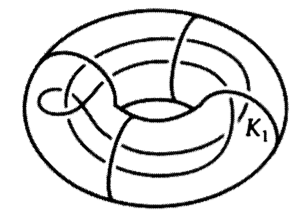
\includegraphics[width=0.5\textwidth] {05.png}
\end{center}

\item Demostrar que la suma conexa de dos nudos $3$-coloreables es un nudo $3$-coloreable.
\end{enumerate}



\begin{figure}[!h]
\centering
\begin{tikzpicture}%[scale=0.75]
\begin{knot}[consider self intersections=true,
%flip crossing=1,
flip crossing=2,
flip crossing=3,
flip crossing=5,
only when rendering/.style={
}]
\strand (0,0) .. controls +(-2,2) and +(3,-3) .. (5,5)
.. controls +(-3,3) and +(-3,0) .. (5,2) 
.. controls +(-3,3) and +(-3,0) .. (0,0) 
%.. controls +(4,0) and +(-3,0) .. (-8,-3)
%.. controls +(3,0) and +(-4,0) .. (-7,2)
;
\end{knot}
\end{tikzpicture}
\end{figure}


\end{document}
